\chapter{Konzeption technischer Umsetzung}\label{chapter:tanforderungen}
Das Ziel des folgende Kapitel ist es zu erläutern wie auf Baisis der aufgestellten gesetzlichen und funktionalen Anforderungen ein der Zielsetzung dieser Arbeit entsprechenden Messanger Dienst erstellt werden kann. Das im folgenden Kapitel erstellte Konzept zur Umsetzung des Dienstes soll als Leitfaden für die reale Erstellung des Messangers dienen. 

\section{Erörterung eines geeigneten Frameworks}\label{chapter:kr}
Um die Umsetzbarkeit der aufgestellten Anforderungen an den Messanger Dienst in einem realistischen und ökonomischen Rahmen zu halten wird davon abgesehen ein komplett neues Messanger System von Grund auf Aufzubauen. Es ist wesentlich effizienter die ENtwicklung des Messangers auf einem bestehenden Framwork aufzubauen, welches sich den Anforderungen entsprechend Anpassen lässt. Das folgende Kapitel beschäftig sich mit Frameworks, welche für die aufgabe in Frage kommen, damit anschließend das Konzept zur Umsetzung des Messangers auf baisis des Ausgewählten Frameworks durchgeführt werden kann. 

\subsection{Auswahl möglicher Framworks}\label{chapter:am}

\subsection{Vorstellung des Matrix Frameworks}\label{chapter:vdmf}
Matrix ist ein offener Standard und ein Kommunikationsprotokoll für  Echtzeitkommunikation. Matrix besteht von Haus aus aus einem opensource Backend, welches über eine http API ereicht werden kann und die Kernfunktionen des Dienstes bereitstellt. Matrix bietet ebenfalls ein opensource Frontend welches ein User Interface bereitstellt über welches via der http API mit dem Backend kommuniziert werden kann. Somit stellt Matrix ein vollständiges, exemplarisches, opensource Backend und Frontend die Implementierung des Dienstes. Ein weiteres Alleinstellungsmerkmal von Matrix gegenüber anderer Standards ist zum einen, dass es mit einem besonderen Fokus auf Sicherheit entwickelt wurde und eine vollständig End zu End verschlüsselte Kommunkation  erlaubt, zum anderen dass es dezentralisert betrieben werden kann. Die Bedeutung der dezentraliserung für die Umsetzung des Dienstes wird in späteren Kapiteln noch weiter erläutert.

Das Matrix-Projekt wurde von einer gemeinnützigen Stiftung mit Sitz in Großbritannien mit dem Ziel ins Leben gerufen, ein Framework für dezentrale Open-Source-Messaging-Dienste mit den Schwerpunkten Sicherheit, Datenschutz und Anpassungsfähigkeit zu entwickeln. Heute bietet Matrix eine robuste Codebasis zum Einrichten benutzerdefinierter Messaging-Dienste und bietet Element eine ergänzende Slack-ähnliche Benutzeroberfläche.

Aufgrund seiner hohen Sicherheitsstandards und seines dezentralen Ansatzes wurde Matrix  von der französischen Regierung ausgewählt, um die Basis für eine sichere Instant Messenger-App zu schaffen und eine bessere Kommunikation in und zwischen verschiedenen Abteilungen der Regierung zu ermöglichen. Neben der französischen Regierung wählte auch die deutsche Bundeswehr Matrix als Basis für die Entwicklung eines internen Kommunikationsinstruments.

\subsubsection{Matrix Funktionsumfang für den Nutzer}\label{chapter:aemn}
Von Haus aus verfügt Matrix bereits über einen sehr robusten Funktionsumfang, welcher im folgenden vorgestellt wird.
Der Aufbau des Dienstes ist mit dem von Slack vergleichbar. Das bedeutet Chats werden in Einzel/ Gruppenchats und Räume aufgeteilt. Während Chats für den austausch zwischen ausgewählten Personen ausgelegt sind, werden Räume Themen spezifisch angelegt. Räume lassen sich zudem auch öffentlich stellen, sodass sie von anderen Nutzern über eine Suche gefunden werden können. Des weiteren bietet Matrix die Möglichkeit Chats und Räume zu sogenannten Communities zusammenzustellen, welche dabei helfen das Interface übersichtlich zu halten.
Neben der Suche nach Räumen ist Matrix auch in der Lage nach im System hinterlegten Nutzern zu suchen. Die Chats selber bieten die von anderen Messangern wie Slack beretis bekannte funktionen wie das Teilen von Dateien, das senden von Emoticons , das Antworten auf spezifische Nachrichten in Form von Threats oder das Reagieren Auf NAchrichten durch Emoticons. Chats und Räume lassen sich mit einer bereitgestellten Suchfunktion durchsuchen. Räume und Chats verfügen auch über weitreichende Optionen zur Administration, darunter ein robustes System zur Vergabe von Rechten an Nutzer, wie zum Beispiel das Recht darauf Nutzer zum Chat/ Raum hinzu zu fügen oder zu entfernen, das Recht Nachrichten in der entsprechenden Gruppe zu verschicken oder Nachrichten zu löschen. Besonders Relevant für die spätere Konzeption ist auch die Möglichkeit seitens Matrix Nachrichten nur für einen bestimmten Zeitraum zu speichern.

Neben den eigentlichen Chat Funktionen ist Matrix auch in der Lage Video und Audio Telefonate mit einzelpersonen oder Gruppen führen.

Matrix erlaubt es dem Nutzer eine Reihe von Identifikatoren, wie Email oder Telefonnummer im eigenen NUtzerprofil zu hinterlegen, ein Profilbild anzulegen, das erscheinungsbild des Messangers zu personaliseren, einzustellen unter welchen Umständen der NUtzer von Matrix benachrichtig werden möchte, zum Beispiel beim eintreffen einer neuen Nachricht, anzupassen, oder sein Passwort zu ändern.  

\subsubsection{Matrix Netwerktoplogie}\label{chapter:aemn}
Einer der großen alleinstellungs Merkmale des Matrix Frameworks ist der dezentralisierte Aufbau, welcher es erlaubt multiple Matrix Instanzen von einander unabhängig zu betreiben, welche dennoch in der Lage sind, mit einander zu kommunizieren. Ein Netzwerk aus mehreren Matrix Instanzen folgt dabei dem folgenden Aufbau:
% Einfügen einer Grafik
\begin{figure}[htb]
    % Zentrierung
    \centering
    % Einfügen der Datei, mit angepasster Höhe
    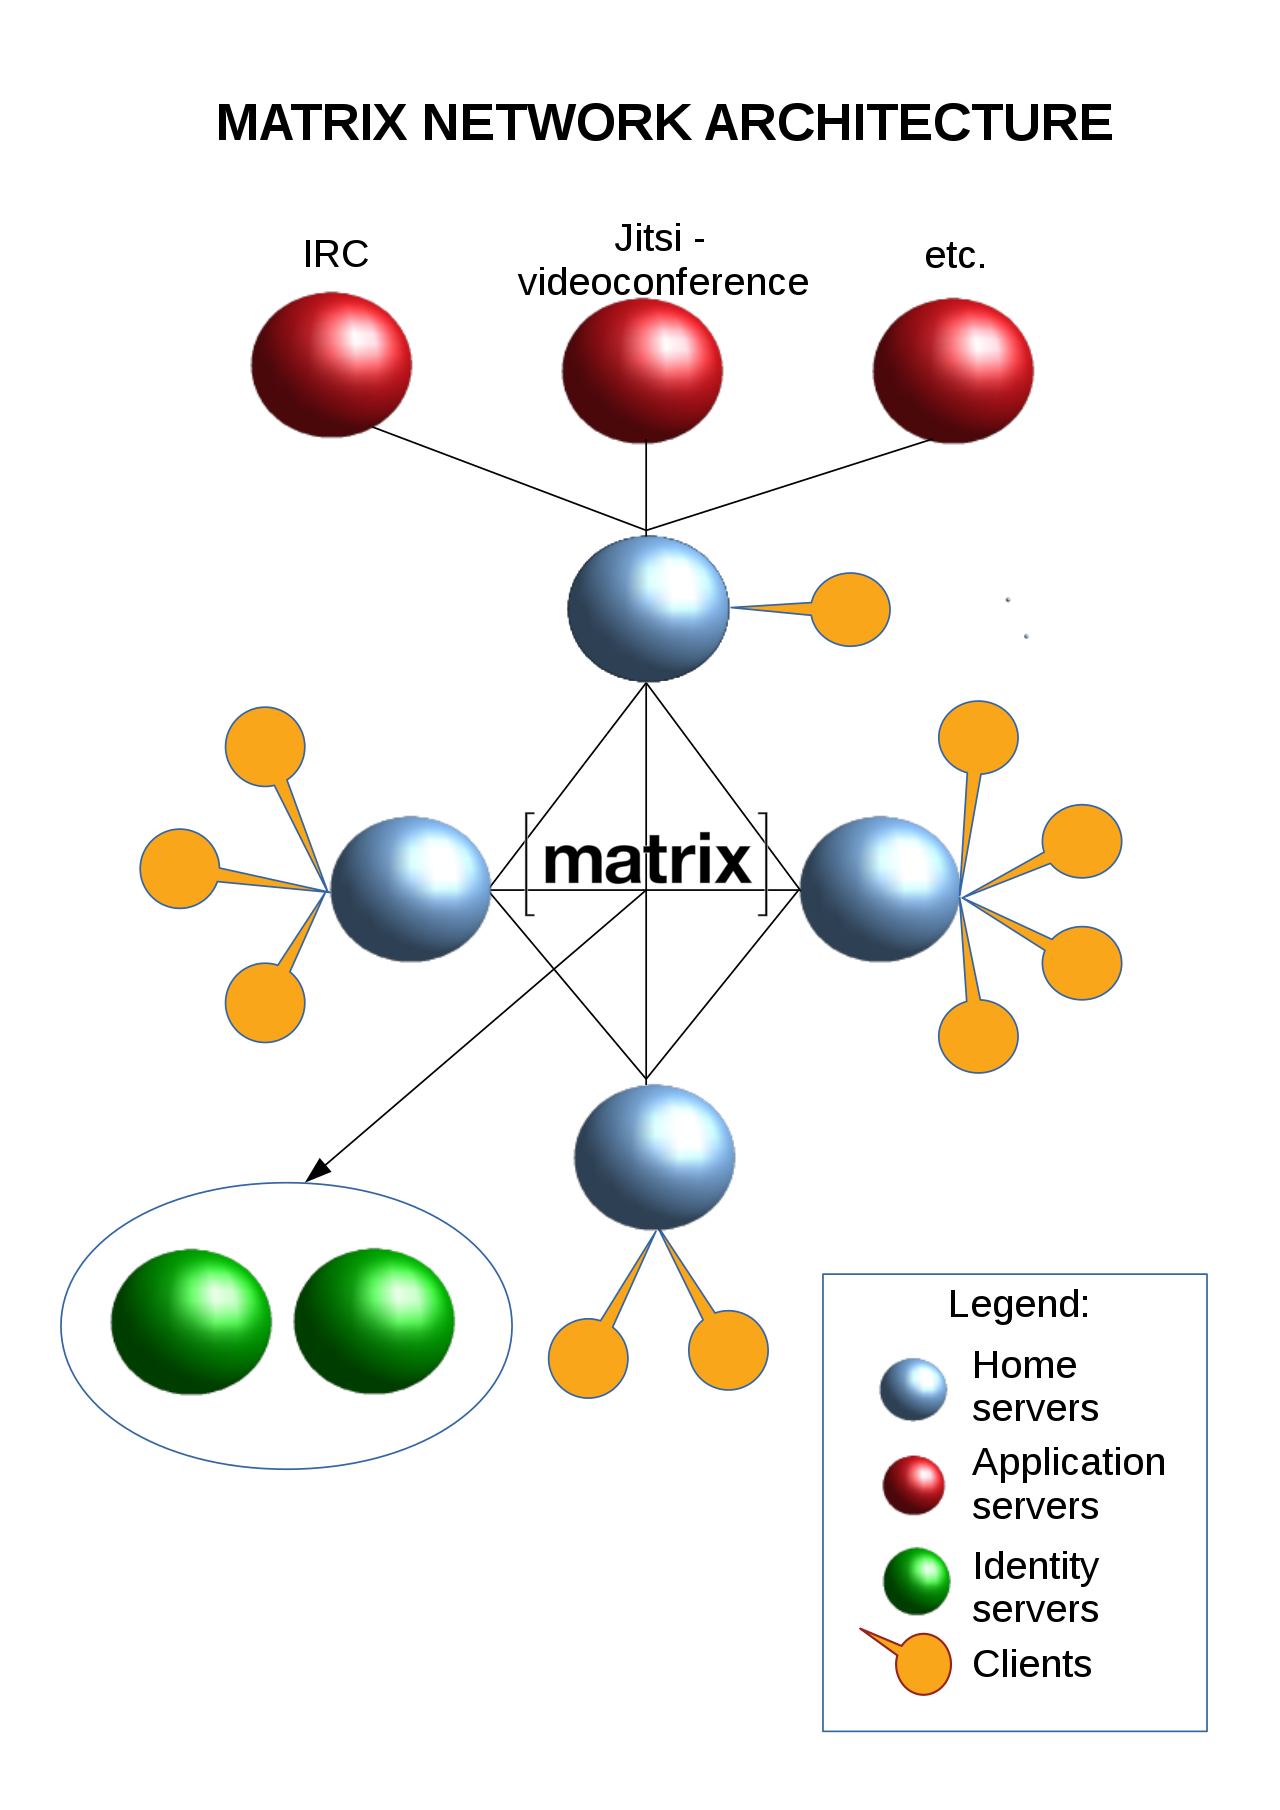
\includegraphics[height=13cm]{graphics/1280px-Diagramme_Matrix_en.png}
    % Titel und Label der Grafik
    \caption[Matrix Netzwerk Architektur]{Matrix Netzwerk Architektur.\footnotemark}
    \label{abb:DHBWLogo}
\end{figure}
\footnotetext{Matrix Netzwerk Architektur Quelle...}
Im Zentrum jeder Matrix Instanz steht der sogenannte Homeserver. Jeder Homeserver stellt dabei einen eigene Instanz des Messangers dar, welcher in Kombination mit einer Datenbank als Speicher und einem Frontend, welches mit den API schnittstellen des Homeservers kommuniziert, betrieben werden kann. Jeder Nutzer (Client) des Matrix Netzwerks ist dabei einem Homeserver zugeordnet, über welchen sein Account verifiziert wird und welcher für die Sicherung seiner Daten und Chatverläufe zuständig ist. Das besondere hierbei ist, dass die Kommunkation innerhalb von Matrix nicht auf einen einzelnen Homeserver beschränkt ist. Durch ein enstprechendes White bzw Blacklisting kann die Kommunkation mit anderen Homeservern erlaubt beziehungsweise eingeschränkt werden. Matrix geht dabei wie folgt vor:
Der Matrix-Standard spezifiziert RESTful-HTTP-APIs für die sichere Übertragung und Replikation von JSON-Daten zwischen Matrix-fähigen Clients, Servern und Diensten. Diese Daten werden mit einer Signatur im Git-Stil signiert, um Manipulationen zu vermeiden. Das Daten Paket wird mit HTTPS verschlüsselt und mit dem privaten Schlüssel des Servers signiert, um Spoofing zu vermeiden.
Die Client sendet dieses Datenpaket dann an den gewälten "Raum" auf dem Matrix Homeserver. Dieser repliziert die Daten dann über alle Matrix-Server, die an diesem "Raum" teilnehmen. Somit ist es möglich gezielt zwischen zwei oder mehr Homeservern zu kommunizieren und nur den inhalt der Chats dieser Räume zwischen den Homeservern auszutauschen, ohne dass sämtliche auf den Datenbanken der Homeserver hinterlegten Chats ausgetauscht werden müssen. Zumdem führt dies auch dazu, dass, sollte ein Homeserver aus Gründen nicht erreibar sein, zum Beispiel durch einen Absturz oder Wartungen an dem System, ist die Kommunkation innerhalb und zwischen den anderen Homeservern des Netzwerks immer noch möglich ist.

FÜr die Verwaltung von Nutzern ist es möglich einen so genanten Identity Server mit dem eigenen Homeserver zu verknüpfen, welcher es erlaubt externe Nutzerverwaltungen zur authentifikation gegenüber dem Homeserver zu Nutzen. Die Basis der Matrixinternen Nutzerverwaltung bildet die sogenannte Matrix user IDs (MXID), welche wie folgt aufgebaut ist "@username:homeserver.tld". Diese ist einzigartig für jeden Nutzer. Darauf aufbauend können Third-party IDs (3PIDs) mit der MXID verbunden werden, wie zum Beispiel eine E-Mail Adresse, eine Handynummer oder ein Display Name, welche die Identifikation einzelner Nutzer vereinfacht. Wird kein Identiy Server mit dem Homeserver Verbunden kann ein Nutzerkonto direkt über den Homeserver erstellt werden. Hierfür kann ein in der Konfiguration des Homeservers festgelegter 3PID in kombination mit einem Passwort angegeben werden, worauf hin der Homeserver den Nutzer anlegt und eine passende MXID erstellt. In der Regel ist es aber wünschenswert eine bereits bestehende Nutzerverwaltung mit dem Homeserver zu verküpfen, da auf diese Weise die Nutzer keine zustzlichen Accounts erstellen müssen, da sie sich über die Nutzerverwaltung authentifizieren können und der Betreiber des Homeservers keine weitere Nutzerverwaltung extra für den Homeserver betreiben muss. Zum verbinden eines Homeservers mit einer Nutzerverwaltung nutzt Matrix eine Reihe von Standartschnittstellen. Ein Beispiel für eine Unterstütze Schnittstelle ist OpenID Connect, ein offener Standart für ein dezentralisiertes authentifikations Protokoll. Andere unterstützte Matrix Schnitstellen sind CAS und SAML .

Neben externen Nutzerverwaltungen können auch andere Module an Matrix angebunden werden. Ein Beispiel für ein solches Modul ist das Videokonferenz Tool Jitsi. Wie auch Matrix basiert Jitsi auf einem Open SOurce Projekt und bietet einen robusten Dienst für Video und Audio telefonate, vergleichbar mit anderen Anbietern auf dem Markt wie Zoom oder Skype. Matrix bietet zwar auch von Haus die Möglichkeit Video und Audio Telefonate zu führen, dabei ist der Funktionsumfang aber deutlich kleiner als der von Jitsi. SOllte also ein großer Fokus bei der verwendung der Platform auf Audio und Videotelefonaten liegen, würde es sinnvoll sein Jitsi als Modul an Matrix anzubinden. Bei Jitsi handelt es sich um nur ein Beispiel für die Möglichkeiten Matrix für den eigenen gebrauch anzupassen.  

Was bedeutet das fürs Krankenhaus...

\subsubsection{Matrix Verschlüsselung}\label{chapter:aemn}
Die End-to-End-Verschlüsselung in Matrix basiert auf den kryptografischen Modell von Olm und Megolm.
 Dadurch können gespeicherte Konversationsdaten nur von Raum-Teilnehmern gelesen werden. Ist dies konfiguriert, sind über Matrix transportierte Daten für Matrix-Server nur als Geheimtext sichtbar. Sie können nur von autorisierten Teilnehmern des Raumes gelesen werden. Die Bibliotheken Olm und Megolm (eine Olm-Erweiterung für größere Chaträume) wurden in einem kryptographischem Review des Unternehmens NCC Group geprüft und die Resultate veröffentlicht. Die Überprüfung wurde finanziert vom Open Technology Fund.

\section{Konzeption des Messangers auf Basis des Matrix Frameworks}\label{chapter:km}
Das folgende Kaptitel zeigt wie mithilfe des Matrix Frameworks ein der Zielsetzung dieser Arbeit entsprechender Messanger konzipiert werden kann. Die Implementierung des Framworks als Basis des Messanger Dienstes erlaubt es einen großteil der imn Kaptiel x festgelegten funktionalen und Gesetzlichen Anforderungen durch eine entsprechende Konfiguration des Frameworks und das aufsetzen eines Matrix Homeservers zu erfüllen. Dieser Vorgang soll im folgenden beschrieben werden, um daraufhin die Konzepte zur Umsetzung von Anforderungen, welche sich nicht dirket über das Matrix Framework abdecken lassen zu erläutern und Abschließend das fertige Konzept anhand der aufgestellten Anforderungen zu validieren.

User Consent Template

\subsection{Umsetzung der funktionalen Anforderungen}\label{chapter:am}
Für das Konzept zur Umsetzung der funktionalen Anforderungen wird eine der standart Installation enstprechende, unkonfigurierte Matrix Instanz vorausgesetzt, für welche ds Webinterface über den Browser im Internet erreichbar ist.  
Der Installationsprozess wird in diesem Kapitel nicht weiter Beschrieben, da es sich hierbei je nach Betriebssystem und Rechenzentrum um einen für jedes Krankenhaus individuellen Prozess handelt und aus diesem Grund eine der Standart Installation entsprechende Matrix Konfiguration auf welcher im folgenden Konzept weiter aufbaut. 

-Nachrichten + Räume möglich 

-Nutzerverzeichnus anbinden 

-

Nach der Insteraltion werden bereits die grundlegenden Funktionen des Messangers in Form eines über den Browser erreichbaren Interfaces zur Verfügung gestellt. Des weiteren ermöglicht der Betrieb von Matrix über einen eigenen Server das beibehalten der Datenhoheit über alle vom Messanger verarbeiteten Daten. 

\subsection{Aufbau des Frontends}\label{chapter:vdmf}
Frontend ist Riot: Opensource code muss wie folgt angepasst werden

Zusätzliche erweiterungen:
Was muss noch zusätzlich eingebaut werden um alle Anfroderungen zu eerfüllen 

Auglsitung vothandener Funktionen und Prüfung mit Anforderungskatalog:
...

\subsection{Prüfung des Konzeptes anhand des Anfroderugnskatalogs}\label{chapter:vdmf}
// Ist das Notwendig ?
Auswertung der Anforderungen und übertragung zu wie man es technsich umsetzen kann.

Sortieren was wirklich schwierig ist umzusetzen und was einfach

Zusammenfassugn mit Fokus auf zu lösende Probleme

//Prototyping: Nur Vorstellung des erstellten Protoypens mit Code im Anhang. Dadurch muss nicht jedes Detail erklärt werden, die These dass es mit Matrix funktioneirt kann aber bestätigt werden.

Lösung der schweren Probleme mit Prototyp mit Matrix + Erlärung 

Kritische betrachtung des Prototypens 

Kritische betrachtung der arbeit

Zusammenfassung und Aussichten
